\documentclass{standalone}
\begin{document}
	\subsection{Pipeline Structure}
	
	In this section I will discuss the general structure of the pipeline, more details about the actual implementation will be given in the next chapter.
	To perform the color quantization I've to found the characteristic color(centroids in the color space) of each tissue and use them for the actual segmentation, dividing the pipeline in two main steps. Before each of these steps we need a preliminary phase that aim to isolate the lung regions in order to exclude the extra lung areas and reduce the false positives and motion artifacts.
	In the end the pipeline structure is divided in three main blocks as we can see in \figurename\,\ref{fig:Pipeline} : 
	\begin{itemize}
		\item \textbf{Pre-Processing and lung extraction}: Preliminary step, involves registration of HU, isolation of lung regions and removal of bronchial structures and air pockets.
		
		\item \textbf{Training} : estimation of the centroids, is performed only ones; 
		
		\item \textbf{Labeling} :  assignment of each voxel to the cluster of the closest centroids, it is the actual segmentation.
	\end{itemize}
	
		
	\begin{figure}[h!]
		\centering 
			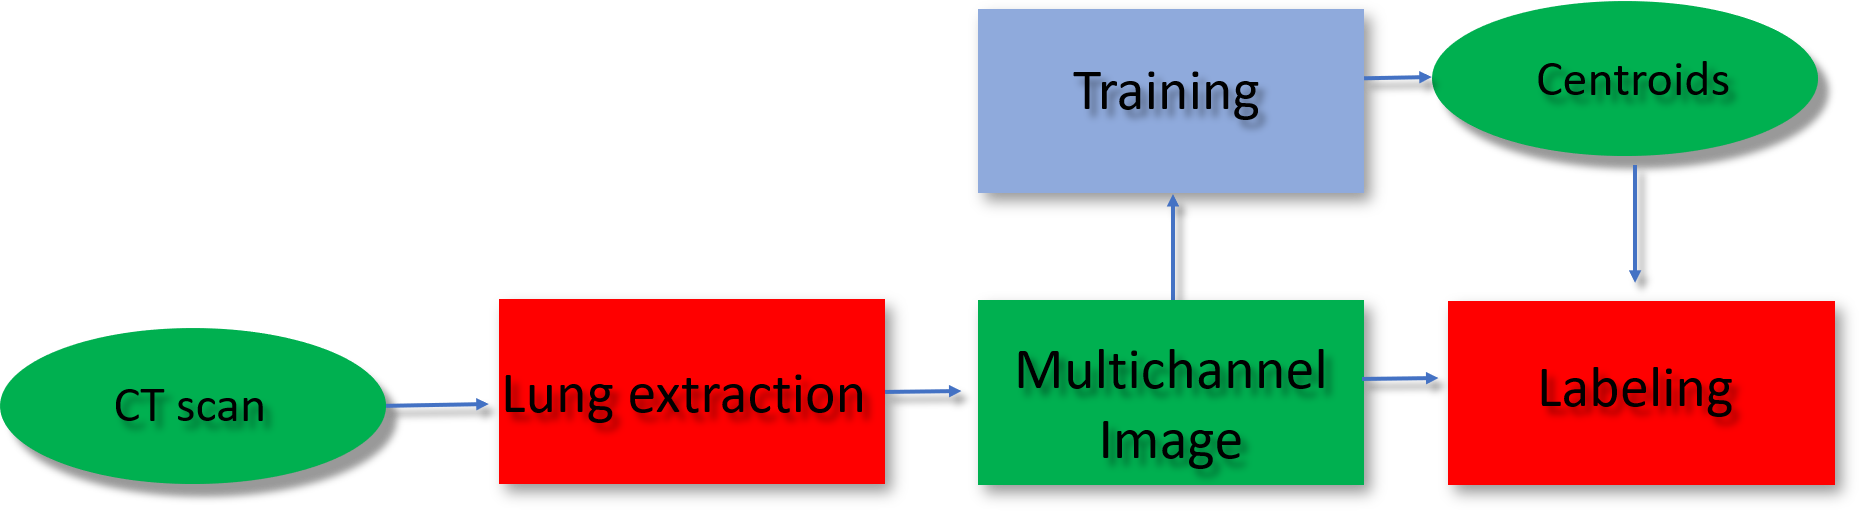
\includegraphics[scale=.65]{Pipeline.png}
		\caption{Flow chart of the main structure of the developed pipeline. The training process, which allows the estimation of the centroids, is performed only one time.}\label{fig:Pipeline}
	\end{figure} 
	
	\subsubsection*{Pre Processing and Lung Extraction}
	
	This preliminary step is performed before both training and labeling; involves the managing of the HU, the isolation of lung regions and the removal of the bronchial structures.\\
	The registration of the HU on a common space in necessary to overcome the issues that may raise from the different padding values and multiplicative constant for HU computation(equation\,\ref{eq:HU}) used by the different manufacturer of the CT scans.\\
	Lung segmentation is pivotal pre-processing step in many image analysis such as classification, identification and classification of lung pathologies~\cite{ART:Johannes}. The lung isolation allow us to found a mask for the lung regions, excluding so all the body regions, the CT tube and the extra-lung organs like intestine and heart, avoiding the fomation of false positives.\\
	Automatic lung segmentation algorithm are typically developed and tested on limited dataset and usually over a limited spectrum of visual variability by containing mainly cases without severe pathologies~\cite{ART:Johannes}. Rule based approach, like thrasholding, region growing, ect, usually fails for CT sans of patients with severe ILD, as we can see in \figurename\,\ref{fig:UNetVSThr}. So, to achieve the lung segmentation I've used  pre-trained UNet~\cite{ART:Johannes}~\cite{REP:lungmask}, that provide a good segmentation of the lung regions. 
	The UNet is a supervised approach, however is used only on this preliminary step, as we will see the identification of infection regions is made with an unsupervised approach.\\
	
	\begin{figure}[h!]
		\centering
		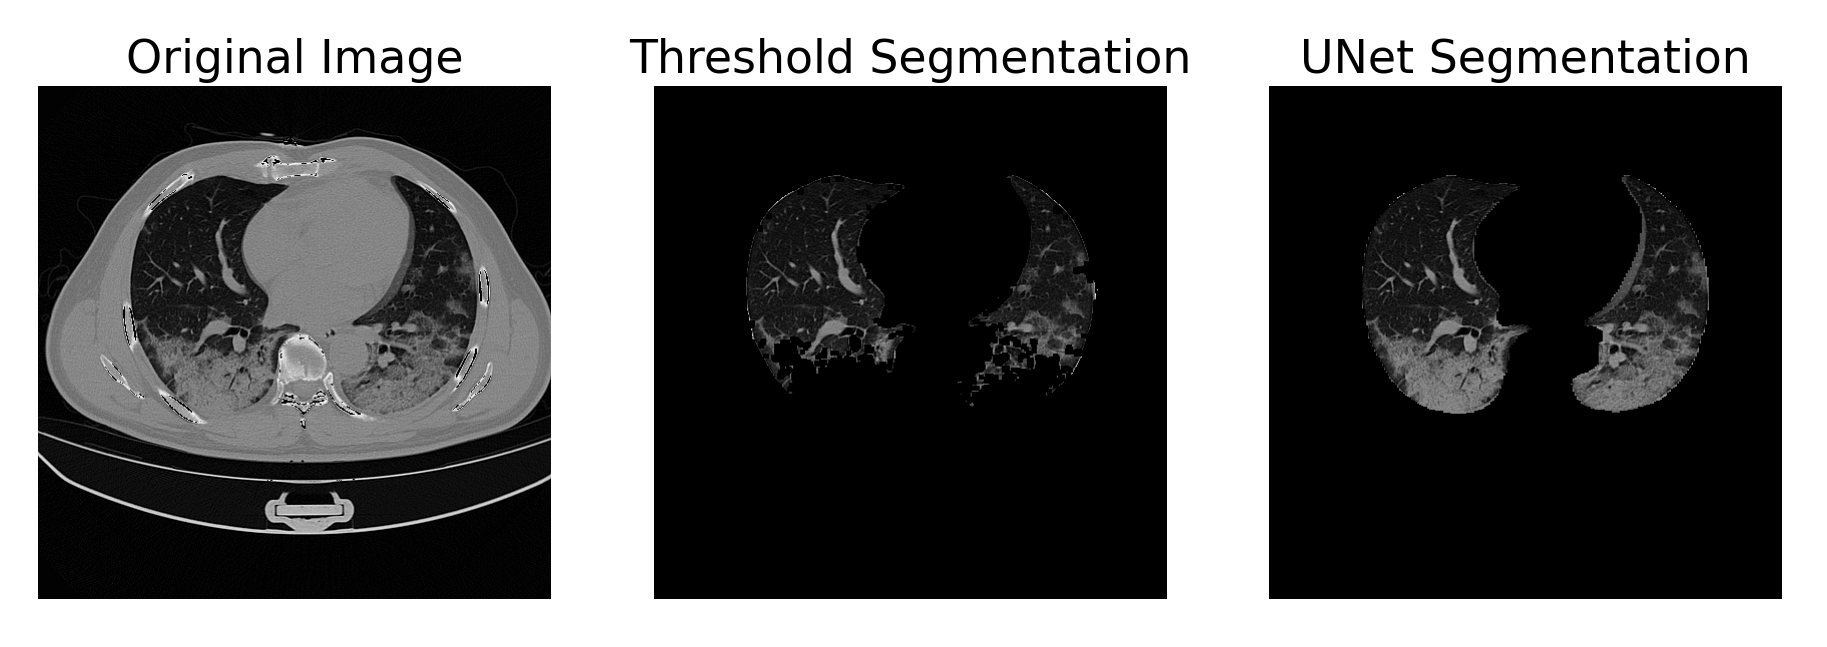
\includegraphics[scale=.5]{UNetVSThr.png}
		\caption{From left to right the original CT scan of a patient with severe ILD, the lung segmented by threshold and connected components, UNet lung segmentation. We can clearly see the missing areas in the fist segmentation, corrected identified in the UNet one.}\label{fig:UNetVSThr}
		
	\end{figure}
	
	This kind of segmentation include in the lung region also motion artifacts and air-pockets, which we will see are the principal cause of false positives. To achieve a better segmentation a refinement process is performed, which aims to remove the main bronchial structures form the selected lung regions. Up to now no motion artifact removal routines is implemented, so we will see that this kind of artifacts wil be the main source of misclassified points. 
	
	\subsubsection*{Training}
	
	This step involves the estimation of the centroids for each tissue. To achieve this purpose we have chose to perform a clustering by using the k-means algorithm. We have to takes into account that the k-means clustering requires an homogeneous representation for each cluster. As we will see we have to manage this problem. Moreover the patient that have a low involvement of lung parenchima have the cluster corresponding to the infection underrepresented, to overcome this issue a careful selection of the patient used for the training was performed. 
	In summary, the implementation of this step involve the building of the multi-channel image, which allow us to takes into account also the neighbouring information, the managing of the over represented clusters  and the actual centroids estimation.

	\subsection*{Labeling}
	
	This step involves the actual segmentation. The script which perform it requires as inputs the CT scans after the lung extraction, and the previously estimated centroids. This block of the pipeline simply assign each voxel to the cluster corresponding to the nearest centroids and the select only the one corresponding to GGO and CS. In this way we are performing a pixel classification by assign regions to a particular labels according only to intensities information, without exploiting spatial information: this allow us to group on the same cluster objects that are spatially disconnected as often happen in medical imaging field.\\
	The distance between voxel color and each centroid is defined as euclidean distance:
	\begin{equation*}
		d(x_j, c_i) = \sqrt{(x_j - c_i)^2}
	\end{equation*} 
	Where $x_j$ is the color vector for the $jth$ voxel and $c_i$ is the $ith$ centroid.\\
	
	To summarize, once the centroids are estimated, the segmentation pipeline will results in $2$ main steps : \textbf{lung extraction} and \textbf{labeling}, as shown in \figurename\,\ref{fig:FinalPipeline} in which we can observe the flowchart of each step with an image that shown the partial results.
	
	\begin{figure}
		\centering
			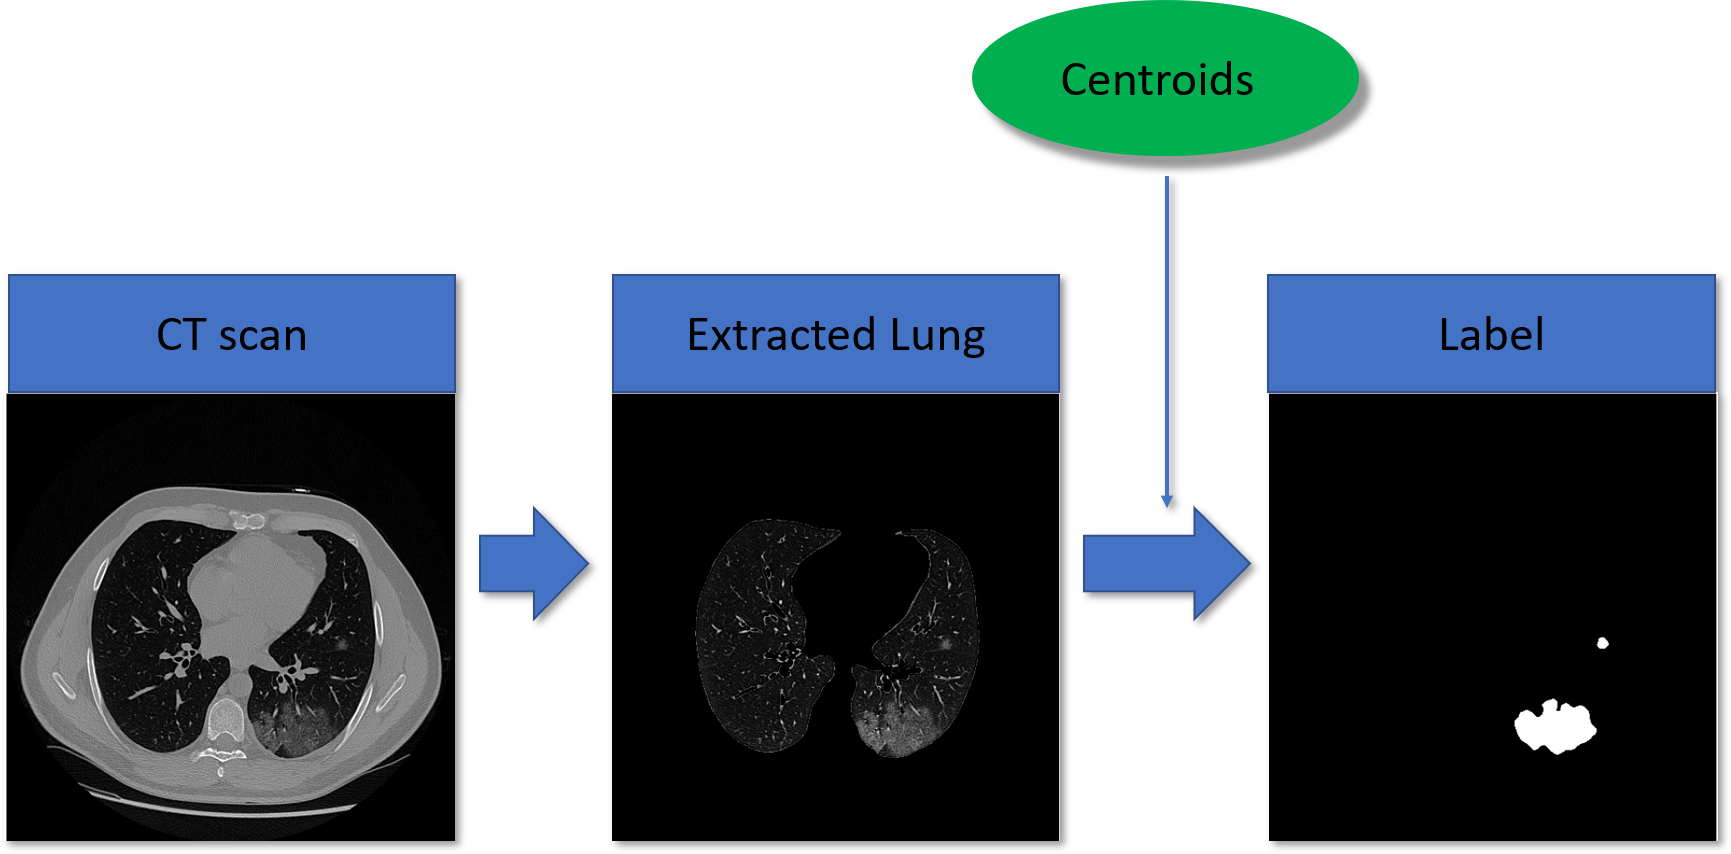
\includegraphics[width=.87\textwidth]{final_pipeline.png}
			\caption{Actual segmentation step, from left to right we can see the input image stack, the isolated lung regions and the final label. To performed the labeling a set of pre-computed centroids was used.}\label{fig:FinalPipeline}
	\end{figure}
	
	
	
\end{document}